%===============================================================================
% LaTeX sjabloon voor de bachelorproef toegepaste informatica aan HOGENT
% Meer info op https://github.com/HoGentTIN/latex-hogent-report
%===============================================================================

\documentclass[dutch,dit,thesis]{hogentreport}

% TODO:
% - If necessary, replace the option `dit`' with your own department!
%   Valid entries are dbo, dbt, dgz, dit, dlo, dog, dsa, soa
% - If you write your thesis in English (remark: only possible after getting
%   explicit approval!), remove the option "dutch," or replace with "english".

\usepackage{lipsum} % For blind text, can be removed after adding actual content

%% Pictures to include in the text can be put in the graphics/ folder
\graphicspath{{graphics/}}

%% For source code highlighting, requires pygments to be installed
%% Compile with the -shell-escape flag!
\usepackage[section]{minted}
\usepackage{listings}
\lstset{
    backgroundcolor=\color{lightgray},  % Set the background color for the snippet
    basicstyle=\ttfamily\small,         % Set the basic style
    breaklines=true,                    % Enable line breaking
    captionpos=b,                       % Set the caption position to bottom
    frame=single,                       
    language=Java,                    % Set the programming language (optional)
    showstringspaces=false,             % Do not show spaces in strings as special characters
    keywordstyle=\color{blue},          % Set keyword style
    stringstyle=\color{red}             % Set string style
}

%% If you compile with the make_thesis.{bat,sh} script, use the following
%% import instead:
%% \usepackage[section,outputdir=../output]{minted}
\usemintedstyle{solarized-light}
\definecolor{bg}{RGB}{253,246,227} %% Set the background color of the codeframe

%% Change this line to edit the line numbering style:
\renewcommand{\theFancyVerbLine}{\ttfamily\scriptsize\arabic{FancyVerbLine}}

%% Macro definition to load external java source files with \javacode{filename}:
\newmintedfile[javacode]{java}{
    bgcolor=bg,
    fontfamily=tt,
    linenos=true,
    numberblanklines=true,
    numbersep=5pt,
    gobble=0,
    framesep=2mm,
    funcnamehighlighting=true,
    tabsize=4,
    obeytabs=false,
    breaklines=true,
    mathescape=false
    samepage=false,
    showspaces=false,
    showtabs =false,
    texcl=false,
}


\author{Can Akkurt}
\supervisor{Mevr. C. Teerlinck}
\cosupervisor{Dhr. F. Iacob}
\title[ Een Proof of Concept Ontwikkeling]%
    {Implementatie van Kunstmatige Intelligentie voor Verbeterde Toeristische Ervaringen bij Historische en Culturele Bezienswaardigheden}
\academicyear{\advance\year by -1 \the\year--\advance\year by 1 \the\year}
\examperiod{1}
\degreesought{\IfLanguageName{dutch}{Professionele bachelor in de toegepaste informatica}{Bachelor of applied computer science}}
\partialthesis{false} %% To display 'in partial fulfilment'
%\institution{Internshipcompany BVBA.}

%% Add global exceptions to the hyphenation here
\hyphenation{back-slash}
%% The bibliography (style and settings are  found in hogentthesis.cls)
\usepackage{biblatex} 
\addbibresource{bachproef.bib}            %% Bibliography file
\addbibresource{../voorstel/voorstel.bib} %% Bibliography research proposal
\defbibheading{bibempty}{}

%% Prevent empty pages for right-handed chapter starts in twoside mode
\renewcommand{\cleardoublepage}{\clearpage}
\renewcommand{\cleardoublepage}{\clearpage}
\renewcommand{\arraystretch}{1.2}

%% Content starts here.
\begin{document}


%---------- Front matter -------------------------------------------------------

\frontmatter

\hypersetup{pageanchor=false} %% Disable page numbering references
%% Render a Dutch outer title page if the main language is English
\IfLanguageName{english}{%
    %% If necessary, information can be changed here
    \degreesought{Professionele Bachelor toegepaste informatica}%
    \begin{otherlanguage}{dutch}%
       \maketitle%
    \end{otherlanguage}%
}{}

%% Generates title page content
\maketitle
\hypersetup{pageanchor=true}

%%=============================================================================
%% Voorwoord
%%=============================================================================



\chapter*{\IfLanguageName{dutch}{Woord vooraf}{Preface}}%
\label{ch:voorwoord}

Voor u ligt mijn bachelorproef getiteld "Implementatie van Kunstmatige Intelligentie voor Verbeterde Toeristische Ervaringen bij Historische en Culturele Bezienswaardigheden". Deze scriptie markeert het einde van mijn studie Computerwetenschappen aan Hogent en vormt tegelijkertijd het begin van een nieuwe professionele reis.

Mijn dank gaat in de eerste plaats uit naar mijn promotor Chantal Teerlinck en co-promotor Franz Iacob, voor hun onschatbare begeleiding en voortdurende ondersteuning gedurende dit project. Hun inzichten en feedback hebben mij geholpen om deze scriptie naar een hoger niveau te tillen. Verder wil ik mijn familie en vrienden bedanken voor hun onvoorwaardelijke steun en aanmoediging tijdens mijn studieperiode.

Een speciaal woord van dank gaat uit naar de vrijwilligers die hun tijd en moeite hebben gestoken in het testen van de proof of concept. Hun waardevolle input en feedback waren cruciaal voor de ontwikkeling en verbetering van de applicatie.

Mijn passie voor technologie ontstond al op jonge leeftijd door een sterke nieuwsgierigheid naar hoe dingen werken en de mogelijkheden van innovatie. Dit leidde tot mijn studie Computerwetenschappen, waar ik een bijzondere interesse ontwikkelde voor kunstmatige intelligentie. Binnen dit domein raakte ik gefascineerd door de mogelijkheden van AI om menselijke ervaringen te verbeteren en te verrijken.

De inspiratie voor deze thesis kwam voort uit mijn liefde voor reizen en het verkennen van culturele locaties. Het idee dat AI kan bijdragen aan een rijkere en informatieve toeristische ervaring, sprak me enorm aan. Door de ontwikkeling van een applicatie die AI en beeldherkenning integreert, wil ik bezoekers van historische en culturele bezienswaardigheden een diepere en zinvollere ervaring bieden.

Dit onderzoek richt zich op het evalueren van verschillende methoden om informatie over culturele objecten en locaties te verkrijgen, met een specifieke focus op de toepassing van kunstmatige intelligentie. De resultaten van dit onderzoek bieden inzicht in de effectiviteit van AI-gestuurde applicaties in vergelijking met traditionele methoden zoals gidsen en online zoekopdrachten.

Ik hoop dat deze scriptie een goed inzicht geeft in de potentie van kunstmatige intelligentie om toeristische ervaringen te transformeren en inspireert tot verdere onderzoek en ontwikkeling op dit gebied.

Dank u voor uw interesse in mijn werk en veel leesplezier gewenst.



Kadir Can Akkurt

Bilzen 23/05/2024
\\
%%=============================================================================
%% Samenvatting
%%=============================================================================

% TODO: De "abstract" of samenvatting is een kernachtige (~ 1 blz. voor een
% thesis) synthese van het document.
%
% Een goede abstract biedt een kernachtig antwoord op volgende vragen:
%
% 1. Waarover gaat de bachelorproef?
% 2. Waarom heb je er over geschreven?
% 3. Hoe heb je het onderzoek uitgevoerd?
% 4. Wat waren de resultaten? Wat blijkt uit je onderzoek?
% 5. Wat betekenen je resultaten? Wat is de relevantie voor het werkveld?
%
% Daarom bestaat een abstract uit volgende componenten:
%
% - inleiding + kaderen thema
% - probleemstelling
% - (centrale) onderzoeksvraag
% - onderzoeksdoelstelling
% - methodologie
% - resultaten (beperk tot de belangrijkste, relevant voor de onderzoeksvraag)
% - conclusies, aanbevelingen, beperkingen
%
% LET OP! Een samenvatting is GEEN voorwoord!

%%---------- Nederlandse samenvatting -----------------------------------------
%
% TODO: Als je je bachelorproef in het Engels schrijft, moet je eerst een
% Nederlandse samenvatting invoegen. Haal daarvoor onderstaande code uit
% commentaar.
% Wie zijn bachelorproef in het Nederlands schrijft, kan dit negeren, de inhoud
% wordt niet in het document ingevoegd.

\IfLanguageName{english}{%
\selectlanguage{dutch}
\chapter*{Samenvatting}
\lipsum[1-4]
\selectlanguage{english}
}{}

%%---------- Samenvatting -----------------------------------------------------
% De samenvatting in de hoofdtaal van het document

\chapter*{\IfLanguageName{dutch}{Samenvatting}{Abstract}}

Deze bachelorproef, getiteld "Implementatie van Kunstmatige Intelligentie voor Verbeterde Toeristische Ervaringen bij Historische en Culturele Bezienswaardigheden", onderzoekt de mogelijkheden van kunstmatige intelligentie (AI) om toeristische ervaringen te verrijken door middel van een innovatieve applicatie. Het doel van deze studie is om te evalueren hoe AI-technologieën kunnen worden toegepast om gedetailleerde en nauwkeurige informatie te verstrekken over culturele objecten en locaties, met als uiteindelijke doel de toeristische ervaring te verbeteren.

De centrale onderzoeksvraag luidt: "Hoe effectief is de implementatie van kunstmatige intelligentie in het verbeteren van toeristische ervaringen bij historische en culturele bezienswaardigheden?" Deze vraag werd onderzocht door een proof of concept (PoC) applicatie te ontwikkelen die AI-gestuurde beeldherkenning en natuurlijke taalverwerking integreert.

De methodologie omvatte het ontwerpen en ontwikkelen van een Android-applicatie die foto's van culturele objecten kan analyseren. De applicatie maakt gebruik van de Google Vision API om objecten te herkennen en ChatGPT 3.5 om contextuele beschrijvingen te genereren. De gegenereerde informatie wordt vervolgens opgeslagen in een SQL-database. De effectiviteit van de applicatie werd getest door middel van een vergelijkende studie waarbij 14 gebruikers de AI-gestuurde methode vergeleken met traditionele methoden zoals het gebruik van gidsen, webzoekopdrachten en QR-codes.

De resultaten van het onderzoek toonden aan dat de AI-gestuurde applicatie in staat was om rijke en nauwkeurige informatie te bieden, wat de gebruikerservaring aanzienlijk verbeterde. Gebruikers waardeerden het gemak en de snelheid waarmee de informatie beschikbaar werd gesteld. Echter, de applicatie had soms moeite met de nauwkeurigheid van de objectherkenning, wat een aandachtspunt is voor toekomstige verbeteringen.

Conclusie: De implementatie van kunstmatige intelligentie in toeristische applicaties biedt aanzienlijke voordelen en heeft de potentie om de manier waarop toeristen informatie verkrijgen te transformeren. Dit onderzoek toont aan dat AI een waardevolle toevoeging kan zijn in de toeristische sector, mits de technologie verder wordt geoptimaliseerd. Toekomstig onderzoek zou zich kunnen richten op het verbeteren van de herkenningsnauwkeurigheid en het uitbreiden van de functionaliteiten van de applicatie om een nog rijkere gebruikerservaring te bieden.


%---------- Inhoud, lijst figuren, ... -----------------------------------------

\tableofcontents

% In a list of figures, the complete caption will be included. To prevent this,
% ALWAYS add a short description in the caption!
%
%  \caption[short description]{elaborate description}
%
% If you do, only the short description will be used in the list of figures

\listoffigures

% If you included tables and/or source code listings, uncomment the appropriate
% lines.
%\listoftables
%\listoflistings

% Als je een lijst van afkortingen of termen wil toevoegen, dan hoort die
% hier thuis. Gebruik bijvoorbeeld de ``glossaries'' package.
% https://www.overleaf.com/learn/latex/Glossaries

%---------- Kern ---------------------------------------------------------------

\mainmatter{}

% De eerste hoofdstukken van een bachelorproef zijn meestal een inleiding op
% het onderwerp, literatuurstudie en verantwoording methodologie.
% Aarzel niet om een meer beschrijvende titel aan deze hoofdstukken te geven of
% om bijvoorbeeld de inleiding en/of stand van zaken over meerdere hoofdstukken
% te verspreiden!

%%=============================================================================
%% Inleiding
%%=============================================================================

\chapter{\IfLanguageName{dutch}{Inleiding}{Introduction}}%
\label{ch:inleiding}

De moderne toeristische sector staat voor de uitdaging om technologisch onderlegde bezoekers te voorzien van rijke, nauwkeurige en relevante informatie over culturele en historische bezienswaardigheden. Traditionele methoden zoals het raadplegen van gidsen, het doorzoeken van webbronnen of het fysiek verkennen van een locatie zijn vaak tijdrovend en kunnen de bezoekerservaring belemmeren door het gebrek aan direct beschikbare en nauwkeurige informatie. Dit onderzoek richt zich op de ontwikkeling en evaluatie van een AI-gestuurde applicatie die deze kloof kan overbruggen door gebruik te maken van geavanceerde beeldherkenning en natuurlijke taalverwerkingstechnologieën.

Het gebruik van kunstmatige intelligentie (AI) in toerisme biedt ongekende mogelijkheden om de bezoekerservaring te verbeteren. Door het integreren van beeldherkenning via de Vision API en contentgeneratie via ChatGPT 3.5, kan een mobiele applicatie toeristen in real-time voorzien van gedetailleerde en accurate informatie over de objecten en locaties die zij bezoeken. Dit onderzoek streeft ernaar om de effectiviteit van een dergelijke applicatie te beoordelen in vergelijking met traditionele methoden zoals webzoekopdrachten, fysieke verkenning en interactie met lokale gidsen of bewoners.

\section{\IfLanguageName{dutch}{Probleemstelling}{Problem Statement}}%
\label{sec:probleemstelling}

Er is een groeiende behoefte aan innovatieve oplossingen die toeristen kunnen helpen bij het verkrijgen van betrouwbare en diepgaande informatie over culturele en historische bezienswaardigheden. Traditionele methoden kunnen vaak niet voldoen aan de behoefte aan direct beschikbare en nauwkeurige informatie. Deze bachelorproef stelt de focus op het onderzoeken van de effectiviteit van een AI-gestuurde mobiele applicatie om deze uitdaging aan te pakken. De doelgroep van dit onderzoek bestaat uit toeristen en culturele instellingen die streven naar verbeterde educatieve en informatieve ervaringen.

\section{\IfLanguageName{dutch}{Onderzoeksvraag}{Research Question}}%
\label{sec:onderzoeksvraag}

De centrale onderzoeksvraag van deze bachelorproef is: "Hoe effectief is een AI-gestuurde applicatie in het verbeteren van de toeristische ervaring door het verstrekken van informatie over culturele en historische bezienswaardigheden in vergelijking met traditionele methoden?" Deze vraag wordt verder opgesplitst in de volgende deelvragen:
\begin{itemize}
    \item Hoe nauwkeurig en relevant is de door de AI-gestuurde applicatie verstrekte informatie?
    \item Hoe gebruiksvriendelijk is de applicatie in vergelijking met andere methoden?
    \item Wat zijn de percepties van gebruikers over de applicatie in termen van toegevoegde waarde en educatieve inhoud?
\end{itemize}

\section{\IfLanguageName{dutch}{Onderzoeksdoelstelling}{Research Objective}}%
\label{sec:onderzoeksdoelstelling}

Het verwachte resultaat van deze bachelorproef is een proof-of-concept van een AI-gestuurde applicatie die in staat is om toeristen te voorzien van nauwkeurige en relevante informatie over culturele en historische bezienswaardigheden. De criteria voor succes omvatten:
\begin{itemize}
    \item Ontwikkeling van een functionerende AI-gestuurde mobiele applicatie.
    \item Integratie van de Vision API voor beeldherkenning en ChatGPT 3.5 voor natuurlijke taalverwerking.
    \item Uitvoering van een vergelijkende studie om de effectiviteit van de applicatie te evalueren ten opzichte van traditionele methoden.
    \item Analyse van gebruikersfeedback en gebruikerstevredenheid.
\end{itemize}

\section{\IfLanguageName{dutch}{Opzet van deze bachelorproef}{Structure of this bachelor thesis}}%
\label{sec:opzet-bachelorproef}

De rest van deze bachelorproef is als volgt opgebouwd:

In Hoofdstuk~\ref{ch:stand-van-zaken} wordt een overzicht gegeven van de stand van zaken binnen het onderzoeksdomein, op basis van een literatuurstudie. Dit omvat een bespreking van bestaande technologieën en methoden voor het verstrekken van toeristische informatie, evenals een beoordeling van de huidige toepassingen van AI in deze context.

In Hoofdstuk~\ref{ch:methodologie} wordt de methodologie toegelicht en worden de gebruikte onderzoekstechnieken besproken om een antwoord te kunnen formuleren op de onderzoeksvragen. Dit hoofdstuk beschrijft in detail de ontwikkeling van de AI-gestuurde applicatie, de integratie van de Vision API en ChatGPT 3.5, en de implementatie van de Java-backend en SQL-database.

In Hoofdstuk~\ref{ch:PoC} wordt de proof-of-concept (PoC) van de AI-gestuurde applicatie gepresenteerd. Dit hoofdstuk bevat een gedetailleerde beschrijving van de architectuur van de applicatie, de datastroom en de integratie van de verschillende componenten. Het biedt ook een overzicht van de uitdagingen en oplossingen die tijdens de ontwikkeling zijn tegengekomen.

In Hoofdstuk~\ref{ch:Het onderzoek} wordt een vergelijkende studie gepresenteerd die de effectiviteit van de AI-gestuurde applicatie evalueert tegenover traditionele methoden voor het verkrijgen van informatie over culturele en historische sites. De methoden omvatten het gebruik van webbronnen, fysieke verkenning ter plaatse, en interactie met mensen in de omgeving. De analyse van de verzamelde gegevens, zowel statistisch als kwalitatief, wordt in detail beschreven.

In Hoofdstuk~\ref{ch:conclusie}, tenslotte, wordt de conclusie gegeven en een antwoord geformuleerd op de onderzoeksvragen. Daarbij wordt ook een aanzet gegeven voor toekomstig onderzoek binnen dit domein. Dit hoofdstuk vat de belangrijkste bevindingen samen, bespreekt de implicaties van deze bevindingen en biedt aanbevelingen voor verdere ontwikkeling en onderzoek.


\chapter{\IfLanguageName{dutch}{Stand van zaken}{State of the art}}%
\label{ch:stand-van-zaken}

% Tip: Begin elk hoofdstuk met een paragraaf inleiding die beschrijft hoe
% dit hoofdstuk past binnen het geheel van de bachelorproef. Geef in het
% bijzonder aan wat de link is met het vorige en volgende hoofdstuk.

% Pas na deze inleidende paragraaf komt de eerste sectiehoofding.

Dit hoofdstuk bevat je literatuurstudie. De inhoud gaat verder op de inleiding, maar zal het onderwerp van de bachelorproef *diepgaand* uitspitten. De bedoeling is dat de lezer na lezing van dit hoofdstuk helemaal op de hoogte is van de huidige stand van zaken (state-of-the-art) in het onderzoeksdomein. Iemand die niet vertrouwd is met het onderwerp, weet nu voldoende om de rest van het verhaal te kunnen volgen, zonder dat die er nog andere informatie moet over opzoeken \autocite{Pollefliet2011}.

Je verwijst bij elke bewering die je doet, vakterm die je introduceert, enz.\ naar je bronnen. In \LaTeX{} kan dat met het commando \texttt{$\backslash${textcite\{\}}} of \texttt{$\backslash${autocite\{\}}}. Als argument van het commando geef je de ``sleutel'' van een ``record'' in een bibliografische databank in het Bib\LaTeX{}-formaat (een tekstbestand). Als je expliciet naar de auteur verwijst in de zin (narratieve referentie), gebruik je \texttt{$\backslash${}textcite\{\}}. Soms is de auteursnaam niet expliciet een onderdeel van de zin, dan gebruik je \texttt{$\backslash${}autocite\{\}} (referentie tussen haakjes). Dit gebruik je bv.~bij een citaat, of om in het bijschrift van een overgenomen afbeelding, broncode, tabel, enz. te verwijzen naar de bron. In de volgende paragraaf een voorbeeld van elk.

\textcite{Knuth1998} schreef een van de standaardwerken over sorteer- en zoekalgoritmen. Experten zijn het erover eens dat cloud computing een interessante opportuniteit vormen, zowel voor gebruikers als voor dienstverleners op vlak van informatietechnologie~\autocite{Creeger2009}.

Let er ook op: het \texttt{cite}-commando voor de punt, dus binnen de zin. Je verwijst meteen naar een bron in de eerste zin die erop gebaseerd is, dus niet pas op het einde van een paragraaf.

\lipsum[7-20]

%%=============================================================================
%% Methodologie
%%=============================================================================

\chapter{\IfLanguageName{dutch}{Methodologie}{Methodology}}%
\label{ch:methodologie}

%% TODO: In dit hoofstuk geef je een korte toelichting over hoe je te werk bent
%% gegaan. Verdeel je onderzoek in grote fasen, en licht in elke fase toe wat
%% de doelstelling was, welke deliverables daar uit gekomen zijn, en welke
%% onderzoeksmethoden je daarbij toegepast hebt. Verantwoord waarom je
%% op deze manier te werk gegaan bent.
%% 
%% Voorbeelden van zulke fasen zijn: literatuurstudie, opstellen van een
%% requirements-analyse, opstellen long-list (bij vergelijkende studie),
%% selectie van geschikte tools (bij vergelijkende studie, "short-list"),
%% opzetten testopstelling/PoC, uitvoeren testen en verzamelen
%% van resultaten, analyse van resultaten, ...
%%
%% !!!!! LET OP !!!!!

In dit hoofdstuk wordt de methodologie beschreven die is gebruikt om de Proof of Concept (PoC) uit te werken en te vergelijken met andere methoden voor het verkrijgen van informatie over historische en culturele locaties. Het doel van dit onderzoek is om te bepalen hoe effectief de AI-gestuurde applicatie is in vergelijking met traditionele methoden zoals het gebruik van webbronnen, fysieke verkenning en interactie met gidsen.

\section{Opzetten PoC}

\subsection{Doel}
Het hoofddoel van deze applicatie is om de ervaring van toeristen bij historische en culturele locaties te verbeteren door een interactieve, intelligente en gebruiksvriendelijke methode te bieden voor het verkrijgen van informatie over artefacten of bezienswaardigheden. Door gebruik te maken van geavanceerde kunstmatige intelligentietechnologieën, waaronder beeldherkenning en natuurlijke taalverwerking, beoogt de applicatie nauwkeurige en contextrijke informatie in realtime rechtstreeks naar het mobiele apparaat van de gebruiker te leveren.

\subsection{Systeemcomponenten}
Het systeem bestaat uit vijf hoofdcomponenten, elk met een cruciale rol binnen de algemene architectuur:

\paragraph{Android-applicatie:}
\begin{itemize}
    \item \textbf{Functionaliteit:} Dit is de gebruikersinterface waarmee toeristen met het systeem interageren. Het stelt gebruikers in staat om foto's te maken van historische artefacten of kenmerken op culturele locaties. Naast het vastleggen van afbeeldingen verzamelt de applicatie ook gebruikersvoorkeuren en feedback om de informatie te personaliseren en de gebruikersbetrokkenheid te vergroten.
    \item \textbf{Gebruikersinteractie:} De applicatie is ontworpen met een eenvoudige en intuïtieve interface, wat zorgt voor gebruiksgemak voor mensen van alle leeftijden. De belangrijkste functies omvatten een cameraknop voor het vastleggen van afbeeldingen, een geschiedenislogboek van opgevraagde items en een informatie weergavegebied waar de door ChatGPT 3.5 gegenereerde inhoud wordt gepresenteerd.
\end{itemize}

\paragraph{Java-backend:}
\begin{itemize}
    \item \textbf{Rol:} Fungeert als de middleware die gegevens van de mobiele applicatie verwerkt en communiceert met zowel de Vision API als ChatGPT 3.5. Het beheert taken zoals beeldvoorverwerking, gegevensversleuteling voor privacybescherming en API-verzoekbeheer.
    \item \textbf{Gegevensverwerking:} Na ontvangst van een afbeelding van de Android-app, voert de backend initiële gegevensverwerking uit om de afbeelding te optimaliseren voor analyse. Dit omvat het aanpassen van de grootte, het filteren en mogelijk het verbeteren van de beeldkwaliteit om de herkenningsnauwkeurigheid te verbeteren.
\end{itemize}

\paragraph{Vision API:}
\begin{itemize}
    \item \textbf{Beeldanalyse:} Maakt gebruik van machine learning-modellen om de ontvangen afbeeldingen te analyseren. Het identificeert objecten, tekst en andere relevante kenmerken binnen de afbeelding. Deze API is gekozen vanwege zijn robuustheid en hoge nauwkeurigheid bij het herkennen van diverse visuele elementen in verschillende omgevingen en lichtomstandigheden.
    \item \textbf{Data-uitvoer:} Levert gestructureerde gegevens over de herkende elementen in de afbeelding, inclusief identificatoren die kunnen worden gebruikt om via de ChatGPT 3.5 API meer gedetailleerde informatie op te halen.
\end{itemize}

\paragraph{SQL-database:}
\begin{itemize}
    \item \textbf{Dataopslag:} Bewaart alle verwerkte afbeeldingen en de bijbehorende AI-gegenereerde beschrijvingen, gebruikersgegevens, en applicatielogboeken. Dit zorgt voor persistentie van de data en maakt het mogelijk om historische gegevens te analyseren en gebruikersspecifieke aanbevelingen te doen.
    \item \textbf{Gegevensbeheer:} Verantwoordelijk voor het efficiënt beheren van gegevensqueries, updates, en verwijderoperaties. Het systeem maakt gebruik van gestructureerde querytaal om interactie met de gegevens te vergemakkelijken, wat bijdraagt aan een snelle en veilige toegang tot informatie.
    \item \textbf{Veiligheid en Privacy:} Implementeert geavanceerde beveiligingsprotocollen zoals data-encryptie en secure access controls om te zorgen dat gebruikersgegevens privé en beschermd blijven tegen ongeautoriseerde toegang.
\end{itemize}

\paragraph{ChatGPT 3.5:}
\begin{itemize}
    \item \textbf{Inhoudsgeneratie:} Ontvangt identificatoren en context van de Java-backend en genereert beschrijvende, informatieve inhoud over de geïdentificeerde objecten of scènes. Dit wordt bereikt door geavanceerde natuurlijke taalverwerkingsmodellen die mensachtige tekst kunnen genereren op basis van de invoergegevens.
    \item \textbf{Interactie:} Bovendien is het systeem ontworpen om te leren van gebruikersinteracties om de reacties te verbeteren en meer gepersonaliseerde informatie te bieden naarmate het meer wordt gebruikt.
\end{itemize}

\subsection{Gegevensstroom}

De gegevensstroom binnen het systeem is zorgvuldig ontworpen om efficiëntie en nauwkeurigheid in de verwerking en het beheer van informatie te garanderen. Hieronder volgt een gedetailleerde beschrijving van elke stap in het proces:

\subsubsection{Stap 1: Afbeelding Vastleggen}
\begin{itemize}
    \item \textbf{Gebruiker Interactie:} De gebruiker neemt een foto met de Android-applicatie. Deze foto kan een historisch artefact of kenmerk zijn binnen een culturele locatie.
    \item \textbf{Data Invoer:} De afbeelding wordt samen met eventuele extra gebruikersinput (zoals voorkeuren en feedback) opgeslagen in het tijdelijke geheugen van de applicatie.
\end{itemize}

\subsubsection{Stap 2: Data Verzending naar Backend}
\begin{itemize}
    \item \textbf{Verzending:} De afbeelding en de bijbehorende data worden via een beveiligde verbinding verzonden naar de Java-backend.
    \item \textbf{Beveiliging:} Tijdens de overdracht zijn de gegevens versleuteld om de privacy en veiligheid van de gebruikersinformatie te waarborgen.
\end{itemize}

\subsubsection{Stap 3: Voorverwerking door Backend}
\begin{itemize}
    \item \textbf{Data-ontvangen:} De Java-backend ontvangt de data en begint met de voorverwerking.
    \item \textbf{Beeldoptimalisatie:} De afbeelding wordt aangepast in grootte, gefilterd en mogelijk verbeterd om de beeldkwaliteit voor analyse te optimaliseren.
\end{itemize}

\subsubsection{Stap 4: Analyse door Vision API}
\begin{itemize}
    \item \textbf{Verzending van Afbeelding:} De geoptimaliseerde afbeelding wordt doorgestuurd naar de Vision API.
    \item \textbf{Analyse:} De Vision API gebruikt machine learning-modellen om de afbeelding te analyseren en relevante kenmerken zoals objecten en tekst te identificeren.
\end{itemize}

\subsubsection{Stap 5: Resultaten Terug naar Backend}
\begin{itemize}
    \item \textbf{Ontvangst van Data:} De Java-backend ontvangt de geanalyseerde gegevens van de Vision API, inclusief identificatoren en metadata van herkende objecten.
\end{itemize}

\subsubsection{Stap 6: Genereren van Inhoud met ChatGPT 3.5}
\begin{itemize}
    \item \textbf{Verzoek om Inhoud:} De Java-backend stuurt de identificatoren en relevante context naar ChatGPT 3.5.
    \item \textbf{Inhoudsgeneratie:} ChatGPT 3.5 genereert beschrijvende, informatieve inhoud op basis van de geïdentificeerde objecten of kenmerken.
\end{itemize}

\subsubsection{Stap 7: Opslag in SQL Database}
\begin{itemize}
    \item \textbf{Dataopslag:} De gegenereerde inhoud samen met de originele afbeelding en de analysegegevens worden opgeslagen in de SQL-database voor toekomstige referentie en analyse.
    \item \textbf{Beveiliging:} Alle opgeslagen data is beveiligd met encryptie en toegangsbeheer om te verzekeren dat alleen geautoriseerde gebruikers toegang hebben.
\end{itemize}

\subsubsection{Stap 8: Weergave aan Gebruiker}
\begin{itemize}
    \item \textbf{Terugkoppeling naar Applicatie:} De gegenereerde inhoud wordt teruggestuurd naar de Android-applicatie.
    \item \textbf{Weergave:} De gebruiker ziet de AI-gegenereerde informatie op het display van de applicatie, samen met eventuele afbeeldingen of relevante data.
\end{itemize}

\pagebreak

\subsection{Architectuurdiagram}

Hieronder wordt het architectuurdiagram gepresenteerd dat de samenhang tussen de verschillende componenten van ons systeem illustreert. De diagram toont de interacties tussen de Android-applicatie, de Java-backend, de Vision API, ChatGPT 3.5 en de SQL-database. Dit diagram is cruciaal voor het begrijpen van de gegevensstroom en de functionaliteit van elke component binnen het systeem.


\begin{figure}[ht]
    \centering
    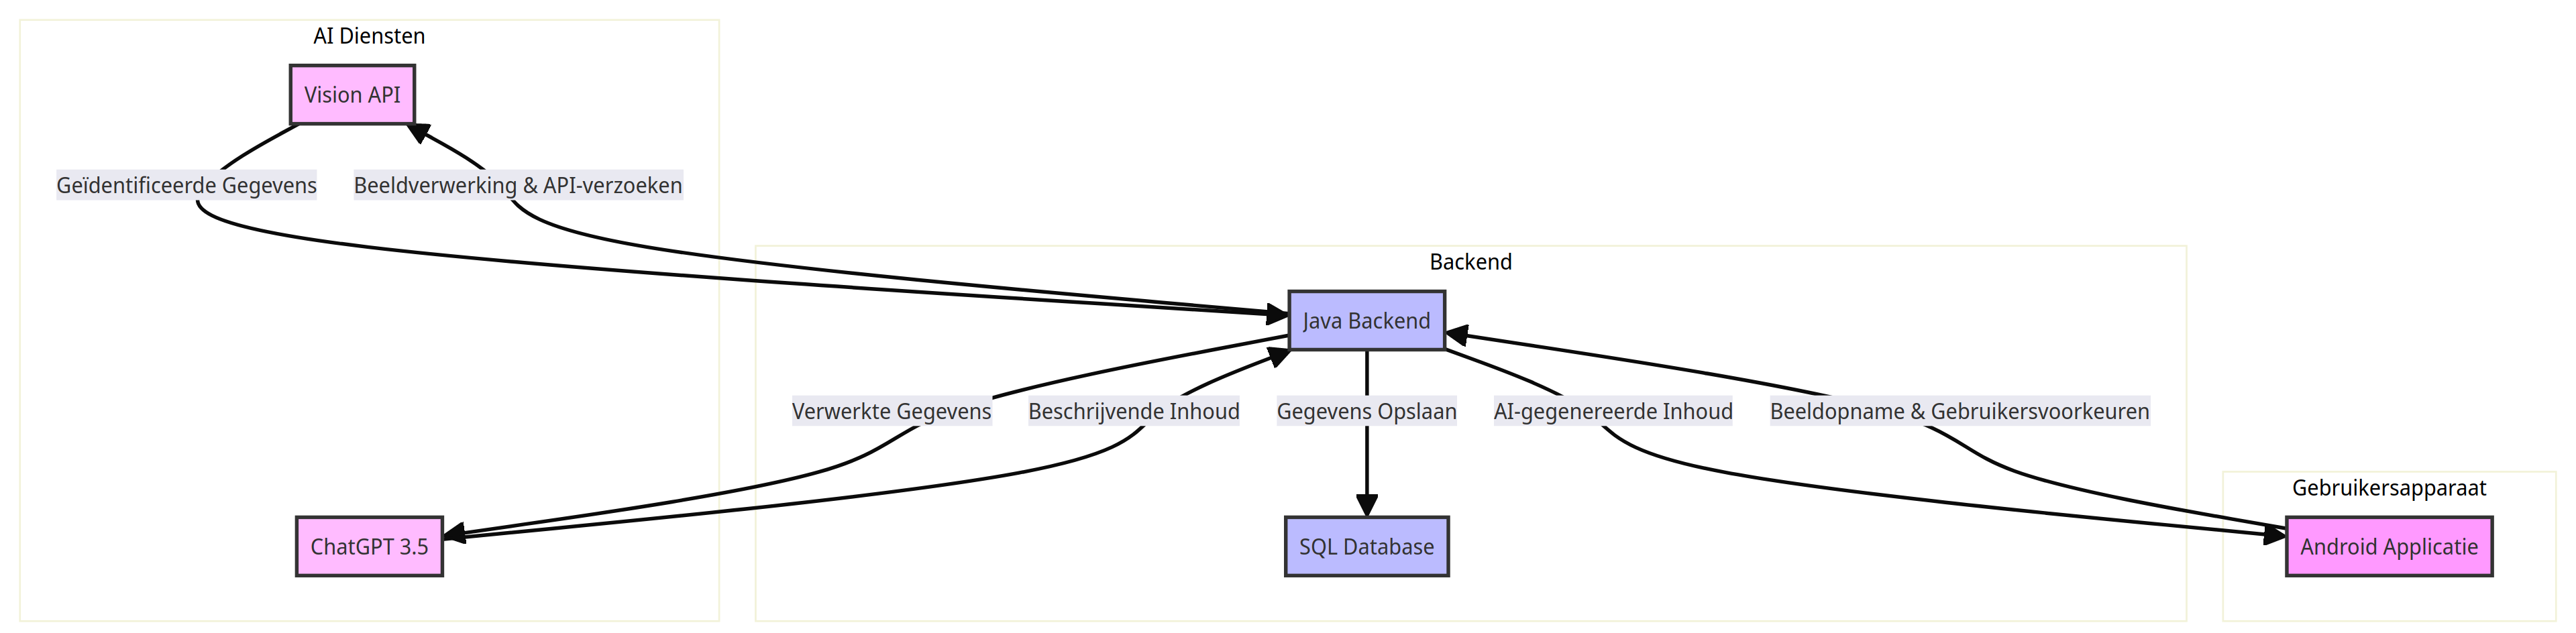
\includegraphics[width=1\linewidth]{ApplicatieArchitectuur.png}
    \caption{Architectuurdiagram}
    \label{fig:example}
\end{figure}

\section{Vergelijking met Andere Methodes}
Om de effectiviteit van de AI-gestuurde applicatie te beoordelen, wordt deze vergeleken met andere traditionele methoden om informatie te verkrijgen over historische en culturele locaties. Deze methoden omvatten het gebruik van webbronnen, fysieke verkenning ter plaatse en interactie met gidsen.

\subsection{Webbronnen}
Het gebruik van zoekmachines en online encyclopedieën zoals Google en Wikipedia is een veelgebruikte methode voor het verkrijgen van informatie. Deze methode biedt uitgebreide en gedetailleerde informatie, maar vereist tijd en inspanning om de meest relevante gegevens te vinden en te verifiëren.

\subsection{Fysieke Verkenning}
Zelfstandige fysieke verkenning van een locatie stelt bezoekers in staat om objecten en kenmerken direct te observeren. Hoewel dit een diepgaande en persoonlijke ervaring biedt, kan het ontbreken van contextuele informatie leiden tot een minder compleet begrip van de culturele en historische betekenis.

\subsection{Interacties met Gidsen}
Het gebruik van professionele gidsen biedt vaak de meest gedetailleerde en contextuele informatie. Gidsen kunnen vragen beantwoorden en aanvullende inzichten bieden die niet gemakkelijk toegankelijk zijn via andere methoden. Deze methode is echter afhankelijk van de beschikbaarheid en kwaliteit van de gids.

\subsection{Beoordelingscriteria}
De vergelijking van de verschillende methoden zal gebaseerd zijn op de volgende criteria:
\begin{itemize}
    \item \textbf{Toegankelijkheid:} Hoe gemakkelijk is het voor gebruikers om toegang te krijgen tot de informatie?
    \item \textbf{Gebruikersvriendelijkheid:} Hoe intuïtief en eenvoudig is de methode in gebruik?
    \item \textbf{Nauwkeurigheid:} Hoe nauwkeurig en betrouwbaar is de verkregen informatie?
    \item \textbf{Gebruikerstevredenheid:} Hoe tevreden zijn gebruikers met de verstrekte informatie en de algemene ervaring?
\end{itemize}

\subsection{Selectie van Testpersonen}
Voor deze vergelijkende studie zijn 14 testpersonen geselecteerd, variërend in leeftijd van 16 tot 50 jaar. Deze diversiteit in leeftijd en achtergrond zorgt voor een representatieve steekproef van de potentiële gebruikers van de applicatie. De testpersonen zijn willekeurig toegewezen aan één van de vier methoden (AI-gestuurde applicatie, webbronnen, fysieke verkenning, en interacties met gidsen) om hun ervaringen en tevredenheid te evalueren. Door deze methoden te vergelijken, wordt beoogd om te bepalen welke benadering het meest effectief is in het leveren van waardevolle en nauwkeurige informatie aan toeristen bij historische en culturele locaties.


%%
%% Het is uitdrukkelijk NIET de bedoeling dat je het grootste deel van de corpus
%% van je bachelorproef in dit hoofstuk verwerkt! Dit hoofdstuk is eerder een
%% kort overzicht van je plan van aanpak.
%%
%% Maak voor elke fase (behalve het literatuuronderzoek) een NIEUW HOOFDSTUK aan
%% en geef het een gepaste titel.


\chapter{PoC}%
\label{ch:PoC}

% TODO: Trek een duidelijke conclusie, in de vorm van een antwoord op de
% onderzoeksvra(a)g(en). Wat was jouw bijdrage aan het onderzoeksdomein en
% hoe biedt dit meerwaarde aan het vakgebied/doelgroep? 
% Reflecteer kritisch over het resultaat. In Engelse teksten wordt deze sectie
% ``Discussion'' genoemd. Had je deze uitkomst verwacht? Zijn er zaken die nog
% niet duidelijk zijn?
% Heeft het onderzoek geleid tot nieuwe vragen die uitnodigen tot verder 
%onderzoek?

\section{Inleiding}
Deze sectie beschrijft de implementatie van het systeem, waarbij wordt ingegaan op de ontwikkeling van de individuele componenten, de integratie van de componenten, en de uiteindelijke inzet van de applicatie. De focus ligt op de technische realisatie van de architectuur zoals beschreven in Hoofdstuk 3.


\section{Android Applicatie}
De Android-applicatie is essentieel voor de interactie met eindgebruikers en is specifiek ontworpen om efficiënt gebruik te maken van de functionaliteiten die moderne smartphones bieden. Het ontwikkelingsproces omvatte verschillende belangrijke aspecten die hieronder in detail worden beschreven:

\begin{itemize}
    \item \textbf{Gebruikersinterface:} De interface is ontwikkeld met een focus op gebruikersvriendelijkheid. De gebruikersinterface maakt gebruik van een modern ontwerp dat responsive is over verschillende schermgroottes en -resoluties. Belangrijke UI-elementen omvatten een interactieve camera-interface, een galerijweergave van recente opnames, en een dynamisch informatiepaneel dat updates ontvangt van de backend.
    
    \item \textbf{Camera-functionaliteit:} De camera-integratie maakt gebruik van de Android Camera2 API, die uitgebreide controle biedt over camerafuncties zoals belichting, focus en resolutie. Dit stelt gebruikers in staat om hoogwaardige afbeeldingen te maken die geschikt zijn voor verder analyse. De app bevat ook functionaliteit om foto's in real-time te beoordelen en te bewerken voordat ze worden verzonden.
    
    \item \textbf{Netwerkcommunicatie:} Om de afbeeldingen te verzenden naar de backend voor verwerking, implementeert de applicatie robuuste netwerkcommunicatiemechanismen. Dit omvat het gebruik van Retrofit voor gestroomlijnde HTTP-verzoeken en responsverwerking. Secure Socket Layer (SSL) encryptie wordt gebruikt om de veiligheid van dataoverdracht te garanderen.
    
\end{itemize}

\subsection{Front-End structuur}

\begin{figure}[h!]
    \centering
    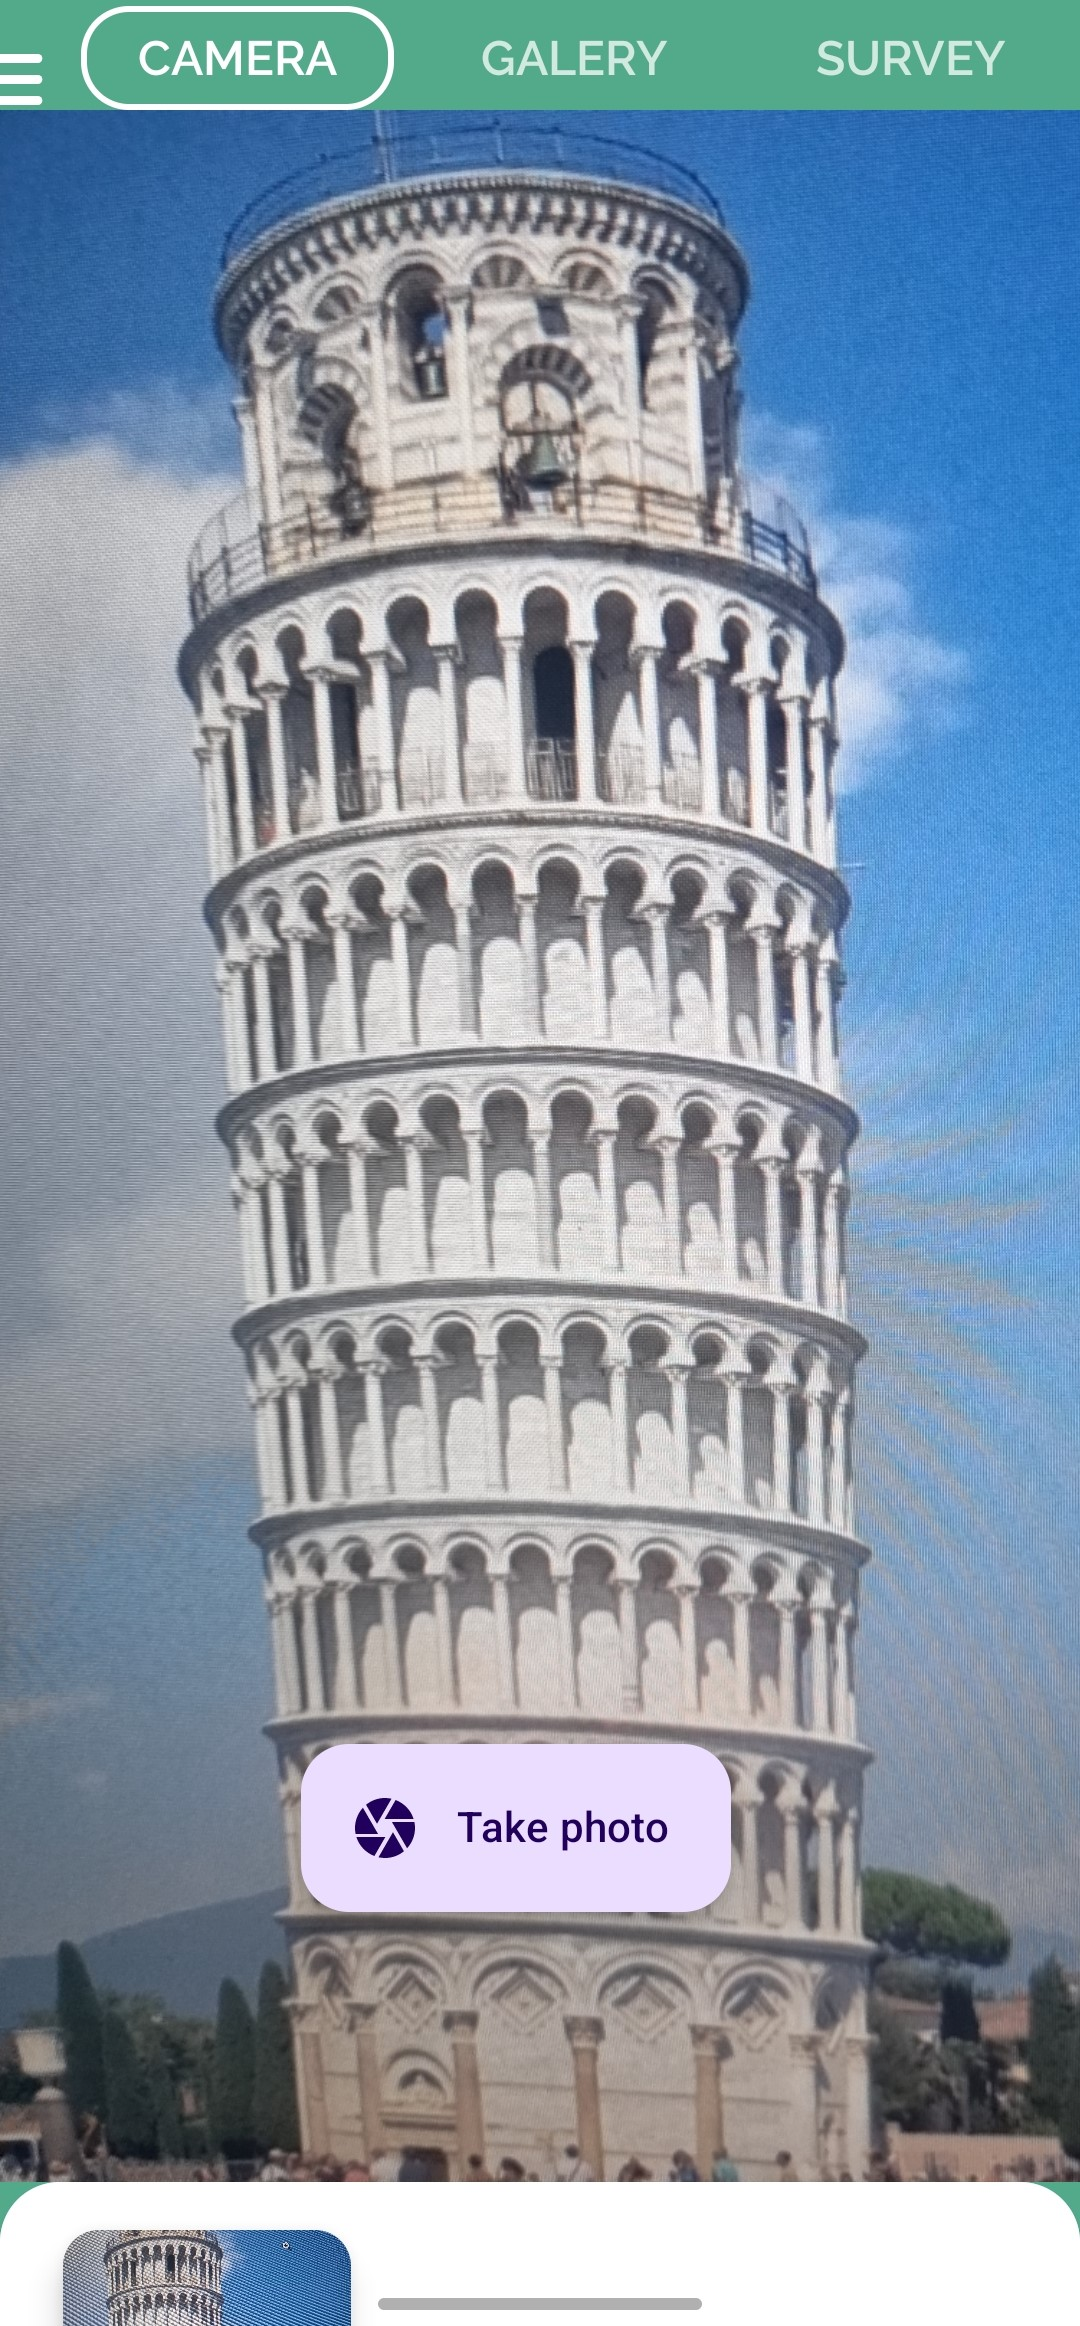
\includegraphics[width=0.5\textwidth]{camera.jpg}
    \captionsetup{justification=centering}
    \caption{Hier kan de gebruiker een foto nemen van de culturele erfgoed.}
    \label{fig:FrontEndCamera}
\end{figure}
\begin{figure}[h!]
    \centering
    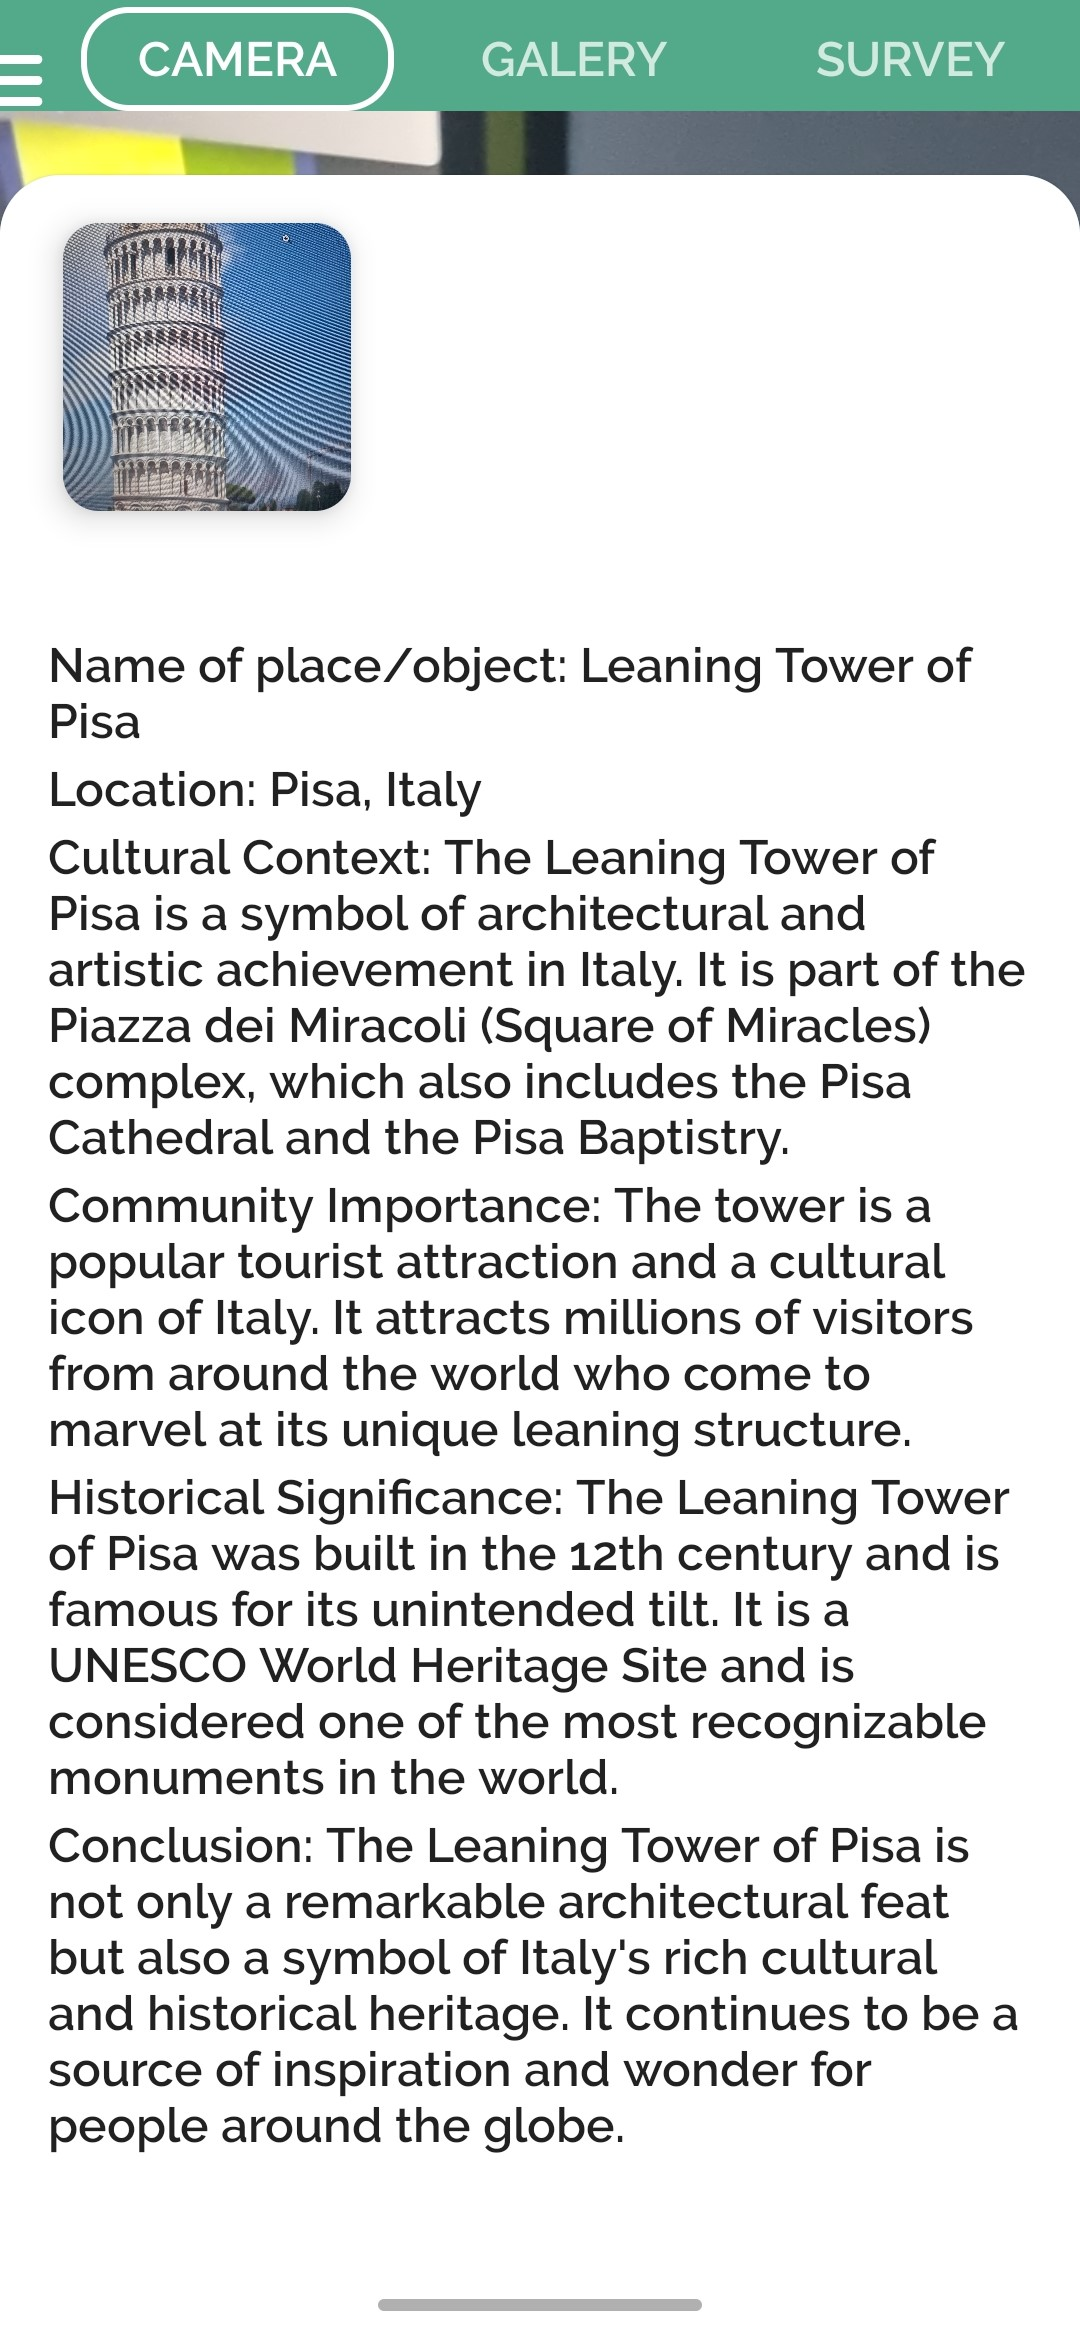
\includegraphics[width=0.5\textwidth]{details.jpg}
    \captionsetup{justification=centering}
    \caption{Hier wordt de door AI gegenereerde tekst weergegeven van het culturele erfgoed waarvoor een foto is genomen.}
    \label{fig:FrontEndCameraDetails}
\end{figure}
\pagebreak
\section{Java Backend}
De backend van het systeem is ontwikkeld in Java, gebruikmakend van het Spring Boot framework, dat efficiëntie en kracht biedt voor enterprise-level applicaties. Deze sectie beschrijft de ontwikkeling, functionaliteiten en belangrijkste technologieën die gebruikt zijn voor de Java-backend.

\begin{itemize}
    \item \textbf{API-ontwerp:} De backend fungeert als de centrale hub voor gegevensverwerking en is verantwoordelijk voor het ontvangen van afbeeldingen van de Android-applicatie, het communiceren met de Vision API en ChatGPT, en het opslaan van gegevens in de SQL-database. RESTful API's zijn geïmplementeerd met Spring Web, wat een gestandaardiseerde manier biedt voor het creëren van eindpunten en het behandelen van clientverzoeken.
    
    \item \textbf{Beeldvoorverwerking:} Voordat afbeeldingen worden doorgestuurd naar de Vision API, voert de backend cruciale voorverwerkingstaken uit zoals het resizen, comprimeren en eventueel het aanpassen van de belichting van de afbeeldingen om de nauwkeurigheid van de beeldanalyse te maximaliseren. Deze processen worden ondersteund door krachtige Java-bibliotheken zoals Java Advanced Imaging (JAI).
    
    \item \textbf{Beveiliging:} Veiligheid is een prioriteit in de ontwikkeling van de backend. Spring Security wordt gebruikt voor het authenticeren en autoriseren van gebruikers, het beveiligen van eindpunten, en het beschermen van gegevensoverdrachten met HTTPS. Bovendien zijn JWT-tokens geïmplementeerd voor een veilige, staatloze gebruikerssessiebeheer.
    
    \item \textbf{Databeheer:} Spring Data JPA wordt gebruikt voor het beheren van databasetransacties en het orkestreren van het data flow proces naar de SQL-database. Het maakt een efficiënte interactie met de database mogelijk via een abstractielaag die automatisch SQL-queries genereert uit repository methoden.
    
\end{itemize}

\pagebreak

\section{Vision API Integratie}
De integratie van Google's Vision API speelt een cruciale rol in de verwerking van afbeeldingen binnen het systeem. Deze sectie bespreekt de implementatie, het gebruik en de belangrijkste voordelen van de Vision API in het kader van dit project.

\begin{itemize}
    \item \textbf{Implementatie:} De Vision API wordt aangesproken via de Java-backend, waarbij gebruik wordt gemaakt van HTTP-verzoeken om afbeeldingen door te sturen en de analysegegevens te ontvangen. Deze integratie vereist nauwgezette configuratie van API-sleutels en verzoeksparameters om de functionaliteit en veiligheid te garanderen.
    
    \item \textbf{Beeldanalyse:} De API is in staat om complexe beelden te analyseren en een breed scala aan visuele gegevens te identificeren, waaronder objectherkenning, tekstextractie en gezichtsdetectie. Deze mogelijkheden zijn essentieel voor het systeem om relevante en nauwkeurige informatie te verstrekken over culturele en historische objecten.
    
    \item \textbf{Gegevensverwerking:} Na ontvangst van de analyse van de Vision API, worden de gegevens verwerkt door de backend. Dit omvat het filteren en formatteren van de data om deze geschikt te maken voor gebruik door ChatGPT voor contentgeneratie.
    
    \item \textbf{Voordelen en Uitdagingen:} Het gebruik van de Vision API biedt significante voordelen, zoals verbeterde nauwkeurigheid en snelheid van gegevensverwerking. Echter, er zijn ook uitdagingen zoals het beheersen van de kosten, het omgaan met de beperkingen van de API-quota, en het verzekeren van de privacy en veiligheid van de verwerkte gegevens.
\end{itemize}
\pagebreak
\subsection{Code}
Hier is een voorbeeld van de code die de Google Vision API gebruikt om webdetecties te vinden. Deze code stuurt een afbeelding naar de Vision API en verwerkt de resultaten van de webdetectie. De volledige documentatie is te vinden bij \autocite{googleVisionAPI}.

\begin{lstlisting}[caption={Voorbeeld van een Java-klasse die de Google Vision API gebruikt om webdetecties te vinden. Gebaseerd op de documentatie van \autocite{googleVisionAPI}},label={lst:googlevisioncode}]
    package org.example;
    import com.google.cloud.vision.v1.*;
    import com.google.cloud.vision.v1.Feature.Type;
    import com.google.protobuf.ByteString;
    import org.springframework.web.multipart.MultipartFile;
    import java.io.IOException;
    import java.util.ArrayList;
    import java.util.List;
    
    public class DetectWebDetectionsImage {
        public static String detectWebDetections(MultipartFile file) throws IOException {
            List<AnnotateImageRequest> requests = new ArrayList<>();
            StringBuilder results = new StringBuilder();
            ByteString imgBytes = ByteString.copyFrom(file.getBytes());
            Image img = Image.newBuilder().setContent(imgBytes).build();
            Feature feat = Feature.newBuilder().setType(Type.WEB_DETECTION).build();
            AnnotateImageRequest request =
            AnnotateImageRequest.newBuilder().addFeatures(feat).setImage(img).build();
            requests.add(request);
            
            try (ImageAnnotatorClient client = ImageAnnotatorClient.create()) {
                BatchAnnotateImagesResponse response = client.batchAnnotateImages(requests);
                List<AnnotateImageResponse> responses = response.getResponsesList();
                for (AnnotateImageResponse res : responses) {
                    if (res.hasError()) {
                        System.out.format("Error: %s%n", res.getError().getMessage());
                        return "Error: " + res.getError().getMessage();
                    }
                    WebDetection annotation = res.getWebDetection();
                    results.append("Entity:Id:Score\n==============\n");
                    annotation.getWebEntitiesList().forEach(entity ->
                    results.append(entity.getDescription()).append(" : ")
                    .append(entity.getEntityId()).append(" : ")
                    .append(entity.getScore()).append("\n"));
                    annotation.getBestGuessLabelsList().forEach(label ->
                    results.append("\nBest guess label: ").append(label.getLabel()).append("\n"));
                    results.append("\nPages with matching images: Score\n==\n");
                    annotation.getPagesWithMatchingImagesList().forEach(page ->
                    results.append(page.getUrl()).append(" : ").append(page.getScore()).append("\n"));
                    results.append("\nPages with partially matching images: Score\n==\n");
                    annotation.getPartialMatchingImagesList().forEach(image ->
                    results.append(image.getUrl()).append(" : ").append(image.getScore()).append("\n"));
                    results.append("\nPages with fully matching images: Score\n==\n");
                    annotation.getFullMatchingImagesList().forEach(image ->
                    results.append(image.getUrl()).append(" : ").append(image.getScore()).append("\n"));
                    results.append("\nPages with visually similar images: Score\n==\n");
                    annotation.getVisuallySimilarImagesList().forEach(image ->
                    results.append(image.getUrl()).append(" : ").append(image.getScore()).append("\n"));
                }
                return results.toString();
            }
        }
    }    
\end{lstlisting}

\section{Output}

Hier is een voorbeeld van een culturele erfgoedsite, het Colosseum in Rome:

\begin{figure}[h!]
    \centering
    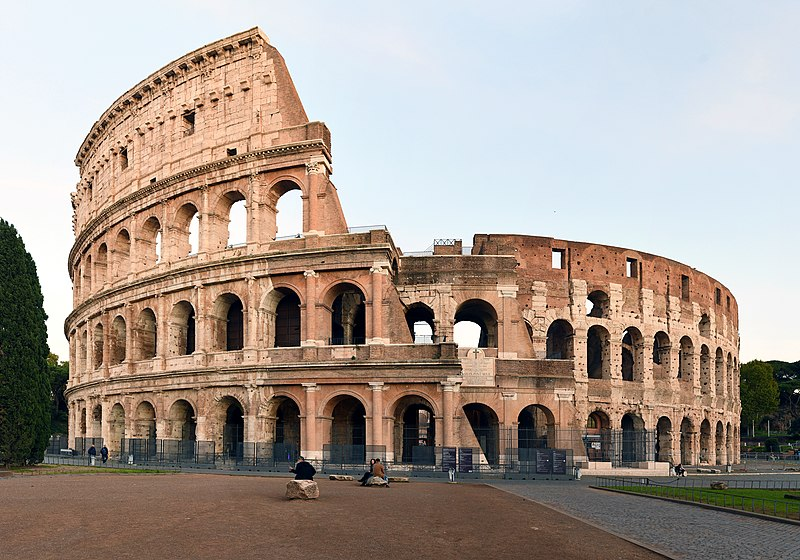
\includegraphics[width=\textwidth]{colosseum.jpg}
    \caption{Het Colosseum in Rome \autocite{wikimediaColosseum}.}
    \label{fig:colosseum}
\end{figure}
\pagebreak

Hieronder zien we de output die verkregen wordt als we de afbeelding in \autoref{fig:colosseum} meegeven aan de Vision API met de code in \autoref{lst:googlevisioncode}.

\begin{lstlisting}[caption={Output vision api},label={lst:outputvisionapi}]
    Entity:Id:Score
    ==============
    Colosseum : /m/0d5qx : 1.7518381
    Ancient Rome : /m/02l341 : 1.1704171
    Roman Forum : /m/0n16t : 1.0100476
    Amphitheater : /m/0f48p : 0.7254882
    Palatine Hill : /m/015376 : 0.679173
    Ancient Roman architecture : /m/0dvg9 : 0.6050097
    Roman amphitheatre : /m/0h1fm4h : 0.5354
    Monument : /m/02ljgl : 0.4356
    : /t/2cs7w02wlkht2 : 0.3742
    Cavea : /m/02drdx : 0.3601
    
    Best guess label: colosseum rome
    
    Pages with matching images: Score
    ==
    https://en.wikipedia.org/wiki/Colosseum : 0.0
    https://www.quora.com/Have-you-been-to-the-Rome-Colosseum-What-did-you-think-when-you-first-saw-it-And-how-did-it-make-you-feel-being-there : 0.0
    https://www.institutodecegosdabahia.org.br/colosseum-ancient-rome-tour-with-gladiator-s-gate-small-dd-EonkR2CW : 0.0
    https://www.quora.com/I-recently-visited-the-Colosseum-and-felt-completely-insignificant-in-its-presence-What-are-other-sites-that-have-made-people-feel-that-way : 0.0
    https://www.italyrometour.com/what-happened-to-the-marbles-that-decorated-the-colosseum/ : 0.0
    https://www.institutodecegosdabahia.org.br/immerse-yourself-in-colosseum-rome-explore-the-iconic-landmark-dd-RWgARpiB : 0.0
    https://aleteia.org/2022/05/04/the-secret-chapel-inside-romes-colosseum/ : 0.0
    https://www.reddit.com/r/todayilearned/comments/18llju0/til_we_dont_know_what_the_romans_called_the/ : 0.0
    https://www.fnh.edu.br/?y=sunrise-at-colosseum-rome-italy-stock-photo-download-image-11-pp-zmZljnuk : 0.0
    https://gbu-hamovniki.ru/announcement/?k=the-colosseum-in-rome-all-things-you-should-know-uu-XR6y1yca : 0.0
    
    Pages with partially matching images: Score
    ==
    https://pbs.twimg.com/card_img/1785266653099438080/bmKNDfRd?format=jpg&name=900x900 : 0.0
    https://media.licdn.com/dms/image/sync/D4D27AQG4QGY9Szh96Q/articleshare-shrink_800/0/1712043042683?e=2147483647&v=beta&t=ezihVY30Lw0-I9UBdYp3_UDIi73UDotxKHSyEFLobv8 : 0.0
    https://i0.wp.com/www.re-thinkingthefuture.com/wp-content/uploads/2022/03/A6454-Keypoints-to-remember-while-understand-roles-of-proportion-in-aesthetics-Image-2.jpg?w=999 : 0.0
    https://lookaside.fbsbx.com/lookaside/crawler/media/?media_id=10223761936025640 : 0.0
    https://howtorhino.com/wp-content/uploads/2023/11/Ancient-Greek-Architecture-22.jpg : 0.0
    https://s2.abcstatics.com/abc/www/multimedia/sevilla/2024/05/08/coliseo-de-roma-RVk0A59wxmwbLirx6Rzm78K-1200x840@diario_abc.jpg : 0.0
    https://i0.wp.com/arteyalgomas.com/wp-content/uploads/2023/03/Coliseo.jpg?resize=840%2C588&quality=89&ssl=1 : 0.0
    https://lookaside.fbsbx.com/lookaside/crawler/media/?media_id=227847066251442 : 0.0
    https://images.techinsider.ru/upload/img_cache/36c/36ccb6f688aa3ab359b22f8084f4cd41_cropped_510x357.jpg : 0.0
    https://www.libremedia.ca/wp-content/uploads/2024/01/1704788233_935_le-classement-des-villes-et-sites-culturels-les-plus-visites.jpeg : 0.0
    
    Pages with fully matching images: Score
    ==
    https://static.android.com.pl/uploads/2023/11/starozytny_rzym_koloseum-scaled.jpg : 0.0
    https://image.spletnik.ru/resize/fit=contain,gravity=0.5x0.5,format=auto,width=1011,height=700,dpr=2/https://image.spletnik.ru/image/2023/06/30/-xw_/original.webp : 0.0
    https://image.spletnik.ru/image/2023/06/30/-xw_/original.webp : 0.0
    http://pic.yupoo.com/fotomag/82123b11/26c91368.jpg : 0.0
    https://upload3.inven.co.kr/upload/2022/07/07/bbs/i13854160493.jpg : 0.0
    https://cdn4.dogonews.com/images/7579050a-0960-470c-bd8c-dae841129103/1920px-colosseo_2020.jpeg : 0.0
    https://assets-global.website-files.com/61d563faa9a56900d65ee25c/62971926a4f2df0997fa5d10_Foto%202.jpg : 0.0
    http://www.apartamento203.com.br/wp-content/uploads/2023/04/Colosseo_2020.jpg : 0.0
    https://lookaside.fbsbx.com/lookaside/crawler/media/?media_id=361667810214259 : 0.0
    https://www.sapiens.cat/uploads/s1/13/88/18/1/roma.webp : 0.0
    
    Pages with visually similar images: Score
    ==
    https://upload.wikimedia.org/wikipedia/commons/thumb/d/de/Colosseo_2020.jpg/1200px-Colosseo_2020.jpg : 0.0
    https://colosseo.it/sito/wp-content/uploads/2018/11/colosseo_esterno.jpg : 0.0
    https://www.pic.int/Portals/5/images/Rome.jpg : 0.0
    https://www.waseda.jp/top/assets/uploads/2024/01/waseda_20240122_img3-360x270.jpg : 0.0
    https://media.beniculturali.it/mibac/files/boards/be78e33bc8ca0c99bff70aa174035096/Luoghi/Parco%20archeologico%20del%20Colosseo%20-%20Colosseo.%20Anfiteatro%20Flavio.jpg : 0.0
    https://cdn.britannica.com/36/162636-131-E4AA93A0/Colosseum-Rome-Italy.jpg : 0.0
    http://pop.h-cdn.co/assets/17/40/3200x1600/landscape-1507135566-colosseum-exterior-inner-and-outer-wall-avl.jpg : 0.0
    https://cdn.getyourguide.com/img/tour/f9964a688f184da5.jpeg/70.jpg : 0.0
    https://st3.idealista.it/news/archivie/styles/highlighted_sm/public/2024-05/images/rome-3550739_1920.jpg?VersionId=rk8PKjYQDOV8smAywUVsKP_M1zZ_9Aux&itok=qUm4fyYX : 0.0
    https://www.odu.edu/sites/default/files/styles/homepage_hero_image/public/images/2022-11/AdobeStock_119146497.jpeg?h=901541b5 : 0.0
\end{lstlisting}

\section{ChatGPT 3.5 Integratie}
De integratie van OpenAI's ChatGPT 3.5 is van cruciaal belang voor het omzetten van visuele data geanalyseerd door de Vision API in gedetailleerde tekstuele beschrijvingen die cultureel en historisch inzicht bieden. Deze integratie maakt gebruik van geavanceerde natuurlijke taalverwerking om informatieve content te genereren die de gebruiker helpt de betekenis en het belang van de bezienswaardigheden te begrijpen.

\subsection{Gegevensverwerking en -integratie}
Na de verwerking van afbeeldingen door de Vision API, waarbij zowel webdetectie als objectherkenning worden toegepast, worden deze data samengevoegd in een gestructureerde output die de basis vormt voor tekstgeneratie. 

\begin{itemize}
    \item \textbf{Data Samenvoeging:} De output van de Vision API, die bestaat uit kenmerken zoals objectherkenning en webdetectiegegevens, wordt gecombineerd tot een enkele samenvattende beschrijving van de afbeelding.
    
    \item \textbf{Prompt Opbouw:} Deze samenvatting wordt dan gebruikt als input voor ChatGPT 3.5 met een specifieke prompt: \texttt "based on this data give information about Name of place/object, Location and Cultural Context, Community Importance, Historical Significance, Conclusion". Deze prompt vraagt ChatGPT 3.5 om uitgebreide informatie te genereren over de naam van de plaats of het object, locatie, culturele context, belang voor de gemeenschap, historische significantie, en een afsluitende conclusie.
\end{itemize}

\subsection{Content Generatie door ChatGPT 3.5}
Op basis van de geformuleerde prompt, genereert ChatGPT 3.5 diepgaande, relevante tekstuele content die rijk is aan culturele en historische informatie.

\begin{itemize}
    \item \textbf{Tekstuele Output:} De gegenereerde teksten bieden uitgebreide informatie die essentieel is voor educatieve en culturele interpretatie door de eindgebruiker.
    \item \textbf{Dynamische Content Aanpassing:} Doorlopende feedback van gebruikers wordt geanalyseerd om de nauwkeurigheid en relevantie van de gegenereerde informatie continu te verbeteren.
\end{itemize}

\subsection{Voordelen en Uitdagingen}
De integratie van ChatGPT 3.5 verrijkt de applicatie aanzienlijk door diepgaande en contextueel relevante beschrijvingen te bieden, maar brengt ook uitdagingen met zich mee zoals de afhankelijkheid van de nauwkeurigheid van de Vision API data en de beheersing van operationele kosten.

\subsection{Implementatievoorbeeld}
Hier krijgen we aan de hand van de input van de Vision API in \autoref{lst:outputvisionapi} deze data van ChatGPT 3.5:

\begin{quote}
“Naam van de Plaats/Het Object
Colosseum (ook bekend als het Flavische Amfitheater).

Locatie
Gelegen in het centrum van Rome, Italië, is het Colosseum een onmiskenbaar herkenningspunt in het historische landschap van de stad, in de buurt van andere belangrijke ruïnes zoals het Forum Romanum en de Palatijn.

Culturele Context
Het Colosseum is een essentieel symbool van de Romeinse ingenieurskunst en cultuur uit de oudheid. Het werd voornamelijk gebruikt voor gladiatorengevechten en openbare spektakels zoals nagespeelde zeeslagen, dierengevechten, executies, reconstructies van beroemde veldslagen en drama’s gebaseerd op klassieke mythologie. Dit amfitheater kon tussen de 50.000 en 80.000 toeschouwers houden, wat de architectonische en technische kunde van de oude Romeinen toont.

Belang voor de Gemeenschap
Het Colosseum blijft een cruciaal herkenningspunt in Rome, niet alleen als een belangrijke toeristische attractie die jaarlijks miljoenen bezoekers trekt, maar ook als een symbool van de rijke historische en culturele erfgoed van Rome. Het staat als een bewijs van de vindingrijkheid van de oude Romeinse architectuur en heeft invloed gehad op het ontwerp van moderne sportstadions.

Historische Betekenis
Gebouwd onder de Flavische keizers tussen 72 en 80 na Christus, weerspiegelt het Colosseum de overgang van de Republiek naar het Keizerrijk in de Romeinse geschiedenis. Het heeft talrijke aardbevingen en diefstallen van stenen doorstaan en blijft grotendeels intact, wat inzicht biedt in de levensstijl, sociale structuur en bestuur van het oude Rome. Het was niet alleen een locatie voor sport en entertainment, maar ook een demonstratie van de macht van het keizerlijke Rome en de sociale stratificatie die heerste in de Romeinse samenleving.

Conclusie
Het Colosseum is niet alleen een architectonisch hoogstandje; het is een cultureel icoon dat de tand des tijds heeft doorstaan, een venster biedend op de oude beschaving van Rome en blijft de esthetiek en functionaliteit van de moderne architectuur beïnvloeden. Het omvat de grandeur van het oude Rome en blijft een centraal onderdeel van de identiteit van Rome en een cruciale locatie voor het begrijpen van de menselijke geschiedenis en cultuur.”
\end{quote}


\chapter{Het onderzoek}%
\label{ch:Het onderzoek}

Dit hoofdstuk presenteert een vergelijkende studie die de effectiviteit van de AI-gestuurde applicatie evalueert tegenover traditionele methoden voor het verkrijgen van informatie over culturele en historische sites. Deze methoden omvatten het gebruik van webbronnen, fysieke verkenning ter plaatse, en interactie met mensen in de omgeving.

\section{Methodologie voor Vergelijkende Studie}
De studie omvatte het verzamelen van gegevens van gebruikers die verschillende methoden gebruikten om informatie over dezelfde culturele bezienswaardigheden te verkrijgen. Elk van deze methoden werd beoordeeld op basis van criteria zoals toegankelijkheid, gebruikersvriendelijkheid, nauwkeurigheid van de informatie, en de algehele gebruikerstevredenheid.

\section{Datacollectie}
Data werden verzameld via enquêtes en directe observatie, waarbij gebruikers werden gevraagd hun ervaringen te documenteren met elke methode. Deelnemers waren een diverse groep die willekeurig werd toegewezen aan een van de methoden, met inachtneming van variabelen zoals leeftijd, achtergrond, en technische vaardigheid.

\subsection{Testpersonen en Dataverzameling}
Voor deze studie werden 14 testpersonen geselecteerd, variërend in leeftijd van 16 tot 50 jaar, met verschillende achtergronden en technische vaardigheden. Deze testpersonen werden willekeurig toegewezen aan een van de vier methoden (AI-applicatie, webzoekopdrachten, fysieke verkenning, en interactie met mensen) om ervoor te zorgen dat de resultaten representatief zijn voor een breed scala aan gebruikers. Data werd verzameld door middel van enquêtes na het gebruik van elke methode en directe observatie tijdens het proces.

\section{Analyse van Resultaten}
De analyse van de verzamelde gegevens is cruciaal voor het bepalen van de effectiviteit van de verschillende methoden om informatie over culturele bezienswaardigheden te verkrijgen. Deze sectie beschrijft de statistische en kwalitatieve methoden die zijn gebruikt om de prestaties van de AI-gestuurde applicatie, webzoekopdrachten, fysieke verkenning en interactie met mensen in de omgeving te evalueren.

\subsection{Statistische Analyse}
Kwantitatieve gegevens, zoals gebruikerstevredenheidsscores, tijdsduur voor het verkrijgen van informatie, en de nauwkeurigheid van de verkregen informatie, werden verzameld en geanalyseerd met behulp van de volgende statistische methoden:
\begin{itemize}
    \item \textbf{ANOVA (Analysis of Variance)}: Gebruikt om te bepalen of er significante verschillen zijn in de gemiddelde tevredenheidsscores tussen de verschillende methoden. Dit helpt bij het identificeren welke methode als het meest bevredigend wordt ervaren door de gebruikers.
    \item \textbf{Chi-kwadraat testen}: Toegepast om te onderzoeken of verschillen in categorieën zoals gebruikersvoorkeuren statistisch significant zijn.
    \item \textbf{Correlatieanalyse}: Uitgevoerd om de relaties tussen de leeftijd en technische vaardigheid van gebruikers en hun voorkeuren voor bepaalde informatieverzamelingsmethoden te beoordelen.
\end{itemize}

\textbf{Resultaten van ANOVA voor Gebruikerstevredenheid}:
\begin{table}[H]
    \centering
    \begin{tabular}{|l|c|c|}
        \hline
        \textbf{Methode}           & \textbf{Gemiddelde Tevredenheidsscore} & \textbf{Standaarddeviatie} \\ \hline
        AI Applicatie              & 4.3                                   & 0.75                      \\ \hline
        Webzoekopdrachten           & 3.8                                   & 0.90                      \\ \hline
        Fysieke Verkenning          & 3.2                                   & 1.10                      \\ \hline
        Interactie met mensen       & 2.6                                   & 1.20                      \\ \hline
    \end{tabular}
    \caption{ANOVA-resultaten voor gebruikerstevredenheid}
    \label{tab:anova-satisfaction}
\end{table}

De ANOVA toonde significante verschillen in tevredenheidsscores tussen de methoden (F(3, 52) = 4.67, p < 0.01). Post-hoc analyse (Tukey's HSD) liet zien dat interactie met mensen significant lagere tevredenheidsscores had vergeleken met de andere methoden.

\textbf{Tijdsduur voor het Verkrijgen van Informatie}:
\begin{table}[H]
    \centering
    \begin{tabular}{|l|c|c|}
        \hline
        \textbf{Methode}           & \textbf{Gemiddelde Tijd (minuten)} & \textbf{Standaarddeviatie} \\ \hline
        AI Applicatie              & 3                                 & 2                          \\ \hline
        Webzoekopdrachten           & 6                                 & 4                          \\ \hline
        Fysieke Verkenning          & 10                                & 7                          \\ \hline
        Interactie met mensen       & 9                                 & 5                          \\ \hline
    \end{tabular}
    \caption{Gemiddelde tijdsduur voor het verkrijgen van informatie}
    \label{tab:time-spent}
\end{table}

\textbf{Resultaten van ANOVA voor Informatienauwkeurigheid}:
\begin{table}[H]
    \centering
    \begin{tabular}{|l|c|c|}
        \hline
        \textbf{Methode}           & \textbf{Gemiddelde Nauwkeurigheidsscore} & \textbf{Standaarddeviatie} \\ \hline
        AI Applicatie              & 3.5                                     & 0.80                      \\ \hline
        Webzoekopdrachten           & 4.2                                     & 1.00                      \\ \hline
        Fysieke Verkenning          & 2.8                                     & 1.20                      \\ \hline
        Interactie met mensen       & 2.4                                     & 1.30                      \\ \hline
    \end{tabular}
    \caption{ANOVA-resultaten voor informatienauwkeurigheid}
    \label{tab:anova-accuracy}
\end{table}

De ANOVA voor informatienauwkeurigheid toonde significante verschillen aan tussen de methoden (F(3, 52) = 5.21, p < 0.01). De nauwkeurigheid van de verkregen informatie werd gemeten door de data die gebruikers verkregen met de verschillende methoden te vergelijken met de juiste data van de culturele bezienswaardigheid waarvan we weten dat deze 100% accuraat is.

\subsection{Kwalitatieve Analyse}
Naast statistische methoden werd er ook een diepgaande kwalitatieve analyse uitgevoerd op de verzamelde feedback en open reacties:

\begin{itemize}
    \item \textbf{Thema-analyse}: Gebruikt om terugkerende thema’s en patronen binnen de gebruikersfeedback te identificeren, wat inzicht geeft in de gebruikerservaringen en percepties van de effectiviteit van elke methode.
    \item \textbf{Inhoudsanalyse}: Toegepast om de diepte en relevantie van de informatie die door elke methode wordt verkregen te beoordelen, en hoe deze informatie bijdraagt aan de verrijking van de culturele ervaring.
\end{itemize}

\textbf{Samenvatting van Kwalitatieve Bevindingen}:

\begin{itemize}
    \item \textbf{AI Applicatie}: Gebruikers waardeerden het gemak en de snelheid van toegang tot informatie, hoewel er meldingen waren van incidenten waarbij de applicatie niet het juiste culturele object identificeerde, wat soms leidde tot verwarring.
    \item \textbf{Webzoekopdrachten}: Gebruikers waardeerden de beschikbaarheid van uitgebreide informatie online, maar vonden het tijdrovend om door verschillende bronnen te bladeren en de nauwkeurigheid te verifiëren.
    \item \textbf{Fysieke Verkenning}: Gebruikers genoten van de ervaring van zelf ontdekken, maar voelden dat ze vaak belangrijke contextuele informatie misten die door gidsen of technologie kon worden verstrekt.
    \item \textbf{Interactie met mensen}: Gebruikers waardeerden de persoonlijke verhalen en tips, maar ervoeren ook inconsistentie in de kwaliteit van de informatie en noemden dat er soms geen mensen beschikbaar waren om te helpen.
\end{itemize}

\subsection{Geïntegreerde Data-analyse}
De resultaten van zowel de statistische als de kwalitatieve analyses werden geïntegreerd om een holistisch beeld te krijgen van de effectiviteit van de verschillende methoden:

\begin{itemize}
    \item \textbf{AI Applicatie}: Scoorde hoog op gemak en snelheid, met gemiddelde tevredenheid en nauwkeurigheid. Gebruikers merkten op dat hoewel de applicatie snel informatie bood, het soms moeite had om het juiste culturele object te identificeren.
    \item \textbf{Webzoekopdrachten}: Bood uitgebreide informatie maar was tijdrovend en soms onnauwkeurig.
    \item \textbf{Fysieke Verkenning}: Werd gewaardeerd voor de ervaring, maar had een lage tevredenheid en nauwkeurigheid vanwege het gebrek aan gedetailleerde informatie.
    \item \textbf{Interactie met mensen}: Had de laagste tevredenheid en nauwkeurigheidsscores vanwege inconsistente informatie en de soms afwezigheid van behulpzame personen.
\end{itemize}


% Voeg hier je eigen hoofdstukken toe die de ``corpus'' van je bachelorproef
% vormen. De structuur en titels hangen af van je eigen onderzoek. Je kan bv.
% elke fase in je onderzoek in een apart hoofdstuk bespreken.

%\input{...}
%\input{...}
%...

%%=============================================================================
%% Conclusie
%%=============================================================================

\chapter{Conclusie}%
\label{ch:conclusie}

% TODO: Trek een duidelijke conclusie, in de vorm van een antwoord op de
% onderzoeksvra(a)g(en). Wat was jouw bijdrage aan het onderzoeksdomein en
% hoe biedt dit meerwaarde aan het vakgebied/doelgroep? 
% Reflecteer kritisch over het resultaat. In Engelse teksten wordt deze sectie
% ``Discussion'' genoemd. Had je deze uitkomst verwacht? Zijn er zaken die nog
% niet duidelijk zijn?
% Heeft het onderzoek geleid tot nieuwe vragen die uitnodigen tot verder 
%onderzoek?

\lipsum[76-80]



%---------- Bijlagen -----------------------------------------------------------

\appendix

\chapter{Onderzoeksvoorstel}
can akkurt 
Het onderwerp van deze bachelorproef is gebaseerd op een onderzoeksvoorstel dat vooraf werd beoordeeld door de promotor. Dat voorstel is opgenomen in deze bijlage.

%% TODO: 
%\section*{Samenvatting}

% Kopieer en plak hier de samenvatting (abstract) van je onderzoeksvoorstel.

% Verwijzing naar het bestand met de inhoud van het onderzoeksvoorstel
%---------- Inleiding ---------------------------------------------------------

\section{Introductie}%
\label{sec:introductie}

Mijn bachelorscriptie zal gaan over het onderwerp "De implementatie van kunstmatige intelligentie (AI) voor het verrijken van de ervaring van toeristen tijdens het bezoek aan historische en culturele locaties". Dit onderwerp wordt geplaatst binnen de veel bredere context van technologische innovatie binnen de toeristenindustrie, waarbij specifiek wordt gekeken hoe AI de interacties tussen bezoekers en andere belanghebbenden op het niveau van attracties kan herdefiniëren.

De primaire doelgroep zou alle belanghebbenden in het veld moeten zijn: van beleidsmakers tot degenen die de managers van historische en culturele sites organiseren, van ontwikkelaars van bijbehorende technologieën tot uiteraard de toeristen zelf. Elk van hen — beleidsmakers, sitebeheerders, technologieontwikkelaars en toeristen — heeft een belang bij het onderwerp: de eersten om manieren bij de hand te hebben om de aantrekkelijkheid en toegankelijkheid van de locaties te verhogen; de tweede om nieuwe toepassingsgebieden voor hun producten te ontwikkelen; en de derde om te zoeken naar verrijkte en gepersonaliseerde ervaringen.

Het probleem dat dit onderzoek probeert te identificeren, is hoe de toepassing van AI specifiek zou kunnen helpen om de ervaring van toeristen die historische en culturele sites bezoeken te verbeteren. Dit leidt tot de hoofdonderzoeksvraag: "Op welke manier kan de toepassing van kunstmatige intelligentietechnologie binnen de erfgoed- en cultuursector bijdragen aan de verrijking van de bezoekerservaring aan historische en culturele site waarden, en hoe kan dat het beste worden geïmplementeerd?"

%---------- Stand van zaken ---------------------------------------------------

\section{State-of-the-art}%
\label{sec:state-of-the-art}


De huidige stand van zaken toont dat AI-technologieën, waaronder machine learning, natuurlijke taalverwerking, en computer vision, reeds worden geïntegreerd in verschillende facetten van de toeristische industrie. Dit varieert van gepersonaliseerde aanbevelingssystemen voor reizigers tot interactieve en augmented reality-toepassingen voor het verrijken van de bezoekerservaring bij culturele en historische sites. Belangrijke publicaties zoals die van \autocite{Zhou2018} benadrukken hoe AI de personalisatie van toeristische ervaringen kan verbeteren, terwijl \autocite{Umerov2023InnovativeDO} de potentie van AI in het verhogen van de toegankelijkheid en het educatieve aanbod van culturele sites verkent.

Desondanks blijven er open vragen en uitdagingen binnen het onderzoeksdomein. De effectieve integratie van AI in de toeristische sector vereist vaak nog verdere verfijning en adaptatie aan de specifieke context van historische en culturele sites. Er is ook een groeiende nood aan empirisch onderzoek dat de impact van AI-toepassingen op de bezoekerservaring kwantificeert.

Mijn onderzoek bouwt voort op deze bestaande literatuur en streeft ernaar om een lacune te identificeren: de directe toepasbaarheid en effectiviteit van AI binnen de niche van historische en culturele toerisme-ervaringen. In tegenstelling tot eerdere studies, die zich mogelijk concentreerden op brede AI-toepassingen in toerisme, zal dit onderzoek specifieke AI-gestuurde interventies en hun directe impact op de bezoeker bij culturele en historische sites analyseren.


% Voor literatuurverwijzingen zijn er twee belangrijke commando's:
% \autocite{KEY} => (Auteur, jaartal) Gebruik dit als de naam van de auteur
%   geen onderdeel is van de zin.
% \textcite{KEY} => Auteur (jaartal)  Gebruik dit als de auteursnaam wel een
%   functie heeft in de zin (bv. ``Uit onderzoek door Doll & Hill (1954) bleek
%   ...'')

%---------- Methodologie ------------------------------------------------------
\section{Methodologie}%
\label{sec:methodologie}

De eerste stap is een uitgebreide literatuurstudie van het huidige onderzoekslandschap, waarbij de toepassingen van AI in de context van toerisme, met name op historische en culturele locaties, worden onderzocht. Dit omvat het identificeren en analyseren van relevante literatuur, technologieën en best practices.
\begin{itemize}
    \item \textit{Doel:} Inzicht verkrijgen in bestaande AI-oplossingen en identificeren van onderzoeksgaten.
    \item \textit{Deliverable:} Literatuuroverzichtsrapport.
\end{itemize}

Ontwikkeling van de AI-toepassing:
In deze fase wordt een AI-prototype ontwikkeld dat de bezoekerservaring verbetert. Hier worden de technologie en methodologieën bepaald en ontwikkeld voor het prototype.
\begin{itemize}
    \item \textit{Doel:} Een functioneel AI-prototype creëren.
    \item \textit{Deliverable:} Werkend AI-prototype.
\end{itemize}

Validatie en Testen:
Het ontwikkelde prototype zal in een experimentele omgeving worden getest om de technische prestaties en gebruikerservaring te beoordelen, inclusief het verzamelen en analyseren van feedback en prestatiegegevens.
\begin{itemize}
    \item \textit{Doel:} De AI-toepassing evalueren en gebruikersfeedback verzamelen.
    \item \textit{Deliverable:} Testrapport en feedbackanalyse.
\end{itemize}

Analyse en Conclusie:
Deze laatste fase biedt een analyse van alle verzamelde gegevens om conclusies te trekken over de efficiëntie en het potentieel van de AI-toepassing. Op basis hiervan worden aanbevelingen voor verder onderzoek en toepassing gegeven.
\begin{itemize}
    \item \textit{Doel:} Conclusies en aanbevelingen formuleren op basis van de analyse.
    \item \textit{Deliverable:} Eindrapport met bevindingen en aanbevelingen.
\end{itemize}

%---------- Verwachte resultaten ----------------------------------------------
\section{Verwacht resultaat, conclusie}%
\label{sec:verwachte_resultaten}

Het doel van deze studie is dus om duidelijk te laten zien op welke mogelijke manieren kunstmatige intelligentie (AI) bezoeken aan culturele locaties aantrekkelijker, informatiever en plezieriger kan maken. We verwachten dat de interactie van alle bezoekers met de tentoonstellingen zal toenemen, dat ze meer zullen leren en met meer voldoening de locatie zullen verlaten, omdat AI deel uitmaakte van hun ervaring. Dit zal zeer waardevolle informatie zijn voor mensen die verantwoordelijk zijn voor de marketing van deze sites, aangezien het de praktische voordelen van het gebruik van AI illustreert. De resultaten, mochten deze tegen de verwachtingen in gaan, zullen onze ogen openen voor de redenen, wat leidt tot bevindingen en ons helpt om nog meer te begrijpen over het potentieel van AI in toerisme. Deze studie is bedoeld om duidelijk te maken hoe AI enorm kan bijdragen aan de ervaring van het verkennen van cultureel erfgoed.



%%---------- Andere bijlagen --------------------------------------------------
% TODO: Voeg hier eventuele andere bijlagen toe. Bv. als je deze BP voor de
% tweede keer indient, een overzicht van de verbeteringen t.o.v. het origineel.
%\input{...}

%%---------- Backmatter, referentielijst ---------------------------------------

\backmatter{}

 %% Add Some space between the bibliograpy entries
\printbibliography[heading=bibintoc]

\end{document}
